%% USE one of these:
%% * the first when using pdflatex, which directly typesets your document in the
%%   chosen pdf/a format and you want to publish your thesis online,

%% * the second when you want to print your thesis to bind it, or
%% * the third when producing a ps file and a pdf/a from it.
%%
\documentclass[english, 12pt, a4paper, sci, utf8, a-1b, online]{aaltothesis}

\usepackage{graphicx}
%% Math fonts, symbols, and formatting
\usepackage{amsfonts,amssymb,amsbsy,amsmath,amsthm,enumitem}
\usepackage[parfill]{parskip}
\usepackage{hyphenat}
% \usepackage[style=ieee]{biblatex}
% \addbibresource{zotero.bib}

\hyphenpenalty=10000
\tolerance=1000

%% added by advisor
\usepackage{xcolor}
\newtheorem{theorem}{Theorem}
\newtheorem{lemma}[theorem]{Lemma}
\newtheorem{corollary}[theorem]{Corollary}
\theoremstyle{definition}
\newtheorem{definition}{Definition}
\theoremstyle{remark}
\newtheorem{remark}{Remark}


\newcommand{\fda}[1]{{\color{red} \textbf{Francesco}: #1}}

\newcommand{\TODO}{{\color{red} \textbf{TODO!} }}
\newcommand{\note}[1]{{\color{purple} \emph{#1} }}


%% THESIS INFO
\degreeprogram{Computer Science}

\major{Computer Science}

\code{SCI3028.kand}

\univdegree{BSc}

\thesisauthor{Peik Etzell}

\thesistitle{Coordinated multi-robot motion planning: An overview}

\place{Espoo}

\date{\today}

\supervisor{Professor Eero Hyvönen}

\advisor{Postdoctoral researcher \\Francesco d'Amore}

\uselogo{aaltoRed}{''}

%% THE ENGLISH ABSTRACT:
%% Thesis keywords:
\keywords{}

%% The abstract text. This text is included in the metadata of the pdf file as well
%% as the abstract page.
\thesisabstract{
TODO
}

%% Copyright text. Copyright of a work is with the creator/author of the work
%% regardless of whether the copyright mark is explicitly in the work or not.
%% You may, if you wish, publish your work under a Creative Commons license (see
%% creativecommons.org), in which case the license text must be visible in the
%% work. Write here the copyright text you want. It is written into the metadata
%% of the pdf file as well.
%% Syntax:
%% \copyrigthtext{metadata text}{text visible on the page}

\copyrighttext{Copyright \noexpand\copyright\ \number\year\ \ThesisAuthor}
{Copyright \copyright{} \number\year{} \ThesisAuthor}


\begin{document}

%% Create the coverpage
\makecoverpage


%% Typeset the copyright text.
%% If you wish, you may leave out the copyright text from the human-readable
%% page of the pdf file. This may seem like a attractive idea for the printed
%% document especially if "Copyright (c) yyyy Eddie Engineer" is the only text
%% on the page. However, the recommendation is to print this copyright text.
\makecopyrightpage


%% ENGLISH ABSTRACT
%% All the details (name, title, etc.) on the abstract page appear as specified
%% above.
\begin{abstractpage}[english]
    \abstracttext{}
\end{abstractpage}

%% Force new page so that the Swedish abstract starts from a new page
\newpage

%% SWEDISH ABSTRACT.
\thesistitle{}
\supervisor{Professor Eero Hyvönen} 
\advisor{Postdoctoral researcher Francesco d'Amore}
\degreeprogram{Datateknik}
\major{Datateknik}
\keywords{}
\begin{abstractpage}[swedish]
TODO
\end{abstractpage}


% %% PREFACE
% %% This section is optional.
% \mysection{Preface}

% \vspace{5cm}
% Espoo, \today

% \vspace{5mm}
% {\hfill Peik Etzell \hspace{1cm}}

\newpage


%% TABLE OF CONTENTS
\thesistableofcontents

% \setlength{\parindent}{0}

\clearpage
\section{Introduction}
\section{Introduction}
\subsection{Background}

Robotic motion planning is a field of research in theoretical computer science which has been deeply studied. It focuses on designing and studying algorithms for making robots get from one point to another safely (without colliding) and efficiently (minimizing some properly defined cost function) \cite{mit/chosetPrinciplesRobotMotion2005}.

Robots are modeled in a vast number of ways, which differ in terms of shapes, sizes and kinematics: some warehouse robots can be modeled to move in two dimensions only, while flying drones can be seen as moving in three dimensions.

Robotic arms that move an end-effector are often modeled in six dimensions: three spatial ones and three for orientation. These robotic arms often have so-called kinematic redundancy, meaning they have more degrees of freedom than strictly necessary \cite{robo/ChiaveriniOM16}. Kinematic redundancy increases the fault-tolerance and dexterity of the robot, and makes it possible to re-adjust while hold the same end-effector pose, but it also increases the complexity in motion planning as poses can have different alternative joint configurations \cite{robo/ChiaveriniOM16}. Kinematic redundancy enables the arm to re-adjust while holding the same end-effector pose, which helps dexterity and fault-tolerance, but also increases complexity in planning, as poses can have different alternative joint configurations \cite{robo/ChiaveriniOM16}.

There are many different environments in which robots exist. Assembly line robots have a fairly static environment, well defined start and end positions, and a clear and safe path between them. Robotic vacuum cleaners on the other hand need to map their environment and make decisions dynamically, as furniture, people and pets can change places from time to time. Some robots need to work together; multi-robot systems can be found in warehouses \cite{robo/ParkerRS16}, where parallel motion is highly desirable, but past research has focused mostly on algorithms moving robots one-by-one \cite{siamcomp/DemaineFKMS19}.

\subsection{Parallel robots}

The field of coordinated motion planning for parallel robotics has seen a lot of research in recent years, with algorithms tackling different problems in the field. 

The many real world scenarios to be studied led to the formulation of different problems. The goal is to move the robots from their starting positions to their target positions without colliding with other robots. Without accounting for collisions, finding a solution would of course be trivial, as robots could move straight to their targets. There are two different general types of motion problems: finding a collision-free schedule transforming a workspace from a starting configuration to a target configuration is called a \emph{motion planning problem}, while determining if such a schedule exists is called the \emph{mover's problem} \cite{siamcomp/HopcroftW86}. 

After executing a valid schedule, all robots will have moved from their starting positions to their target positions, and all target positions are occupied by a robot.

Some variations to this motion problem exist: in its \emph{labeled} formulation, robots are unique, and are assigned specific target locations to move to. This problem formulation is the most studied \cite{fun/BrockenHKLS21}. In its \emph{unlabeled} formulation, robots are instead indistinguishable from each other, and targets can be occupied by any robot. In 2014, \cite{ijrr/SoloveyH14} introduced a generalization of labeled and unlabeled problems: in a \emph{(k-)colored} problem, the robots are partitioned into $k$ colors or groups, and each have to move to a target location with the same coloring. \emph{Labeled} and \emph{unlabeled} are then extremes of the \emph{colored} problem formulation: $k=1$ gives an unlabeled problem, as all robots are of the same color, while $k=n$ gives all robots their own unique color. 

% The problem has multiple variations: \refactor{we}{something else}
% in the unlabeled formulation of the problem, we do not care which robot gets to which target position, only that all target positions get occupied. 
% \TODO in the labeled formulation, robots and target positions have labels...
% In case we want to move specific robots to specific targets, we have a labeled problem, where robots and target positions each have labels, such that target positions contain a robot with the same label at the end. 
% Note that such labels can be unique or not, and some works distinguish between these cases: for example, \cite{demaineCoordinatedMotionPlanning2019} considers \emph{unlabeled, colored} and \emph{labeled} as variations on the problem, where \emph{labeled} means unique labels, and \emph{colored} is a generalization of the unlabeled and labeled variants: multiple robots (and targets) can have the same color, and the targets are only to be matched up with robots of the same color. \TODO explicit extreme
% Thus both the unlabeled and labeled formulations can be modeled as specific cases of the colored one.

Real robots are physically three-dimensional objects, but they are mostly restricted to two dimensions in multi-robot applications. There are some works exploring higher dimensions: \cite{arobots/TurpinMMK14}, but current works are quite focused on the two-dimensional setting. Reasons for this might be ease of visualization and thus understanding, simpler algorithms, real world applicability or something else.

The problem can also be modeled both in the continuous or discrete space. In a discrete model, the workspace is modeled as a grid, which can then be handled using graph theory, with grid cells being nodes that the robots occupy and move through.

In a continuous model, the robots can in theory be modeled as close to reality as wanted, but the increased complexity seems to not be worth it. Most current research in motion planning consider only simple shapes, and real warehouse robots also seem to reflect this in their shapes: many are shaped close to circles or squares. Unit radius disks (see \cite{siamcomp/DemaineFKMS19}, \cite{compgeom/BanyassadyBBBFH22}) or unit squares (see \cite{jea/YangV22}) make collision checking a lot simpler: a single distance metric on two robots' centers determines if they are in collision or not. Most continuous space research also study uniform sizes and shapes of robots, but for example \cite{fun/BrockenHKLS21} investigates motion planning of non-uniformly-sized discs.

% Finding the minimum makespan solution to a discrete grid case of the coordinated motion planning problem is found to be NP-hard by \cite{siamcomp/DemaineFKMS19}. \cite{siamcomp/DemaineFKMS19} also conjectures that the continuous formulation of the problem would be at least as hard, but leaves it for future work.
% NP-hardness implies approximation algorithms are justified \cite{siamcomp/DemaineFKMS19}, so research is focused on better approximations and faster computation. 

There is also a distinction between centralized and distributed computing in motion planning. Robots are inherently physically distributed, and a lot of research considers multi-robot systems as a problem of distributed computing. Most research in specifically robotic motion planning uses centralized planning though, where a single entity computes all moves for all robots. Distributed computing considers similar but distinct problems, like \emph{rendezvous} and \emph{exploration}, which are covered in \cite{lncs/FlocchiniGN19}.






\subsection{Thesis objective}

The scope is broad and the problems are varied but related. The goal is to understand and explain current research, what has been done and what is yet to be understood. To achieve this, current state-of-the-art algorithms are compared in terms of their performance in computation and execution, strengths, weaknesses and scalability. How many robots can we support in a real system before motion planning becomes too slow? 




% PRELIMINARIES 
\section{Preliminaries}

\subsection{A discrete grid of robots}

% WORKSPACE 
Let our grid-based workspace be modeled as a graph \( G \coloneqq (V, E)\). 
Let it be a rectangle \(n_1 \times n_2\) where \(n_1, n_2 \geq 2 \text{ and } n_1, n_2 \in \mathbb{N}\). 
Define the vertices as \(V \coloneqq \set{1, 2, \dots , n_1} \times \set{1, 2, \dots , n_2}\).
For any \(v \in V\), let \(v_x, v_y\) be such that \(v = (v_x, v_y)\). 
We will call \(v_x\) the \(x\)-coordinate of \(v\), and \(v_y\) its \(y\)-coordinate.
To measure distance, we use the \emph{Manhattan norm} \(L_1 = \manhattan{v - w} \coloneqq (\abs{v_x - w_x} + \abs{v_y - w_y})\). Using this, the edges can be defined as \(E = \set{(v, w) \mid \manhattan{v - w} = 1 \text{ for } v, w \in V}\). In other words, nodes are only connected to their up to four immediate neighbors in the grid.

% ROBOTS AND CONFIGURATIONS
Let there be \(N \leq \nngrid\)  robots in our workspace. 
We can identify them by a number \(r \in R := \set{1, 2, \dots , N} \subset \mathbb{N}\). 
Let \(\bot\) represent the empty vertices.
A \emph{configuration} is then a mapping \(\conf{} : V \mapsto \set{1, 2, \dots, N, \bot}\) injective upon the robots in \(R\). 
Injectivity implies no two vertices in \(V\) can be occupied at once, so there will always be exactly \((\nngrid - N)\) empty squares in the grid.

% CONFIGURATION INVERSE
The \emph{inverse} of a configuration \(\iconf{}{r} = (x, y), \; r \in R\), is another function mapping robots to their respective positions.
The robots move synchronously and in parallel, up to a single edge at a time. 
A valid (no-collision) configuration \(\conf{1}\) can thus be \emph{transformed} into another valid configuration \(\conf{2}\) in a \emph{single step} if and only if:

% TRANSFORMATION REQUIREMENTS
\begin{align}
	& \parens{\iconf{1}{r} = \iconf{2}{r} \lor (\iconf{1}{r}, \iconf{2}{r}) \in E, \; \forall r \in R}\label{req:limited_movement}\\
	\land & \parens{\nconf{1}{v} = \nconf{2}{w} \Rightarrow \nconf{2}{v} \neq \nconf{1}{w}, \; \forall v, w \in V}\label{req:no_swaps}
\end{align}

In other words, \cref{req:limited_movement} means a robot can stay in place or move to a neighboring square at every step, while \cref{req:no_swaps} forbids two robots from swapping places in a single transformation step (and they can never occupy the same vertex), equivalent to a collision in the real world.

% SCHEDULE
Denote a single transformation step by \(\conf{i} \rightarrow \conf{i + 1}\). 
A \emph{schedule} is a sequence of transformation steps \(S \coloneqq \conf{1} \rightarrow \conf{2} \rightarrow \cdots \rightarrow \conf{k}\). 
A configuration \(\conf{s}\) can be transformed into a configuration \(\conf{t}\) if there exists a schedule \(\conf{s} \rightarrow \conf{s + 1} \rightarrow \cdots \rightarrow \conf{t - 1} \rightarrow \conf{t}\).

% PROBLEM DEFINITION
\begin{definition}\label{def:motion_planning_problem}
	Given a start configuration \(\conf{s}\) and a target configuration \(\conf{t}\) of a workspace, the \emph{motion planning problem} asks to find a schedule that transforms \(\conf{s}\) into \(\conf{t}\).
\end{definition}

Denote the tuple of a workspace and two configurations \(I \coloneqq \parens{G,\ \conf{s},\ \conf{t}}\) as a problem \emph{instance}. 

\begin{remark}\label{remark:reachability}
	For a \(2 \times 2\) square and any \(1 \times n\) rectangle, where \(n \geq 2\), there exist pairs of configurations that are not reachable from each other via any schedule. 
	See \cref{fig:reachability} for an example. For any other rectangular workspace there always exists such a schedule. 
\end{remark}

% IMPOSSIBLE 2*2 SQUARE FIGURE
\begin{figure}[h]
	\centering
	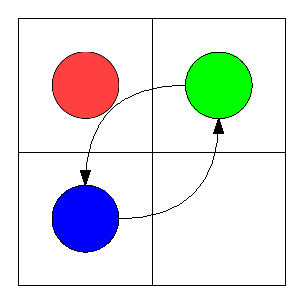
\includegraphics[width=4cm]{include/impossible_2x2.eps}
	\caption{A minimal example of an unsolvable motion planning problem: there exists no valid schedule which swaps the green and blue robots.}\label{fig:reachability}
\end{figure}

% MAKESPAN
\begin{definition}\label{def:makespan}
	The number of single transformation steps in a schedule is called the \emph{makespan} of that schedule.
\end{definition}

\begin{definition}\label{def:optimality}
	Let \(\schedules\) denote the set of all valid schedules for some problem instance \(I\). 
	A schedule \(S_\text{opt}\) is \emph{optimal} with respect to some cost function \(f : \schedules \mapsto \mathbb{N}\) mapping all valid schedules to some integer value if and only if \(f(S) \geq f(\sopt)\) for all such valid schedules \(S \in \schedules\).
\end{definition}

% M3PP -- MINIMUM MAKESPAN MOTION PLANNING PROBLEM
\begin{definition}\label{def:m3pp}
	Let the makespan of a schedule be such a cost function: \(M : S \mapsto \parens{\text{number of steps in S}}\). 
	The \emph{minimum makespan motion planning problem} asks to find an \emph{optimal} schedule with respect to the makespan \(M\) for some input problem instance.
\end{definition}

\begin{remark}
	The \emph{minimum makespan} for any motion planning problem instance \(I \coloneqq \parens{G,\ \conf{s},\ \conf{t}}\) is bounded below by \(\max(\set{\manhattan{\iconf{s}{r}, \; \iconf{t}{r}}, \; r \in R})\).
\end{remark}

\begin{definition}
	Let the aforementioned lower bound to a schedule with makespan \(M\) be denoted by \(L\). 
	The \(\emph{stretch factor}\) for that schedule is then defined as \(\frac{M}{L}\), which is always at least 1. 
\end{definition}

\subsection{Some general notation}

\begin{definition}
	A function \(f(n)\) has an asymptotic upper bound \(g(n)\) if there are some constants \(c \text{ and } n_0\) such that \(f(n) \leq c\cdot g(n),\ \forall n \geq n_0\). 
	It is then denoted as \(f(n) = \mathcal{O}(g(n))\). 
\end{definition}

% Let \emph{A} be some algorithm. 
% \fda{\(A\) is said to run in \emph{polynomial time} ... if the execution of \(A\) by a deterministic Turing machine is done in a polynomial number of steps w.r.t.\ the input bit length... (are yyou sure you want do define this? I think is better to assume it is known)}
% It is \emph{polynomial time} and often said to be \emph{efficient} if the runtime of \emph{A} is bounded by some polynomial function \(T(A) = O(n^c)\) for some constant \(c\).

Let OPT be the optimal (minimum) value of some function \(f\). 
If some algorithm \(A\) can always find a solution that maps to within a \(\rho\)-factor of the optimal value: \(OPT \leq f(x_A) \leq \rho \cdot OPT\), the algorithm is called a \(\rho\)-approximation algorithm. 



% PAPERS 
\note{shorten this title}
\subsection{General approaches to solving multi-robot motion planning problems}
\section{Bounded stretch swarm reconfiguration}

\subsection{Specific preliminaries}

\subsubsection{Definitions}

\begin{definition}
    SAT
\end{definition}

\subsection{About the algorithm(s)}

\subsubsection{High level overview}

\cite{siamcomp/DemaineFKMS19} 


\subsubsection{The discrete grid} 

\begin{theorem}
    The problem of computing an optimal-makespan solution to a parallel motion planning problem on a grid is NP-hard
\end{theorem}

\begin{proof}
    Proof here?
\end{proof}



% CONCLUSIONS
\section{Conclusions}

%% REFERENCES
% \bibliographystyle{aaltosci_t}
\bibliographystyle{ieeetr}
\bibliography{zotero,manual_refs}
% \bibliography{manual_refs}
% \printbibliography

\clearpage

%% ADD POSSIBLE APPENDIX HERE
\thesisappendix

\end{document}
